\chapter*{Opérateurs vectoriels}
\addcontentsline{toc}{chapter}{Opérateurs vectoriels}

\section*{Systèmes de coordonnées}

\begin{figure}[!h]
\center
\hfill
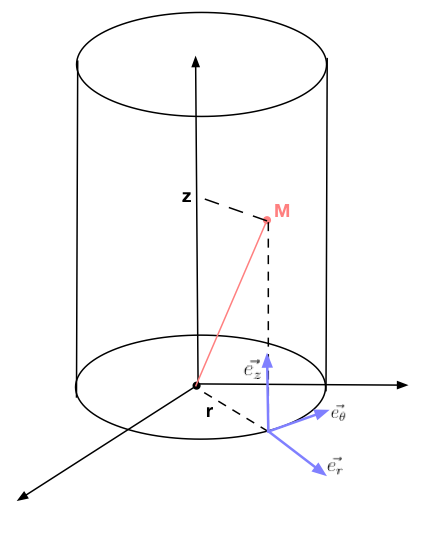
\includegraphics[height=150pt]{source/figures/coordonnees_cyl.png}
\hfill
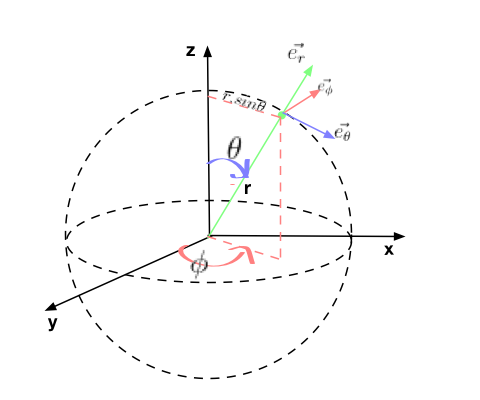
\includegraphics[height=150pt]{source/figures/coordonnees_sph.png}
\hfill
\hfill
\end{figure}

\begin{itemize}
\item cartésiennes : ($\ex$, $\ey$, $\ez$)
\item cylindriques : ($\er$, $\et$, $\ez$)
\item sphériques : ($\er$, $\et$, $\ep$)
\end{itemize}

\section*{Champ scalaire}

\begin{itemize}
\item $U(x,y,z)$
\item $U(r,\theta,z)$
\item $U(r, \theta,\phi)$
\end{itemize}

\section*{Champ vectoriel}

\begin{equation*}
\overrightarrow{A}(x,y,z) = A_x(x,y,z)\ex + A_y(x,y,z)\ey + A_z(x,y,z)\ez
\end{equation*}
\begin{equation*}
\overrightarrow{A}(r,\theta,z) = A_r(r,\theta,z)\er + A_\theta(r,\theta,z)\et + A_z(r,\theta,z)\ez
\end{equation*}
\begin{equation*}
\overrightarrow{A}(r,\theta,\phi) = A_r(r,\theta,\phi)\er + A_\theta(r,\theta,\phi)\et + A_\phi(r,\theta,\phi)\ep
\end{equation*}

\section*{Gradient $\grad$}

Il s'applique à un champ scalaire et est défini par
\begin{equation*}
\d U = \grad U.\overrightarrow{\d l}.
\end{equation*}
En coordonnées cartésiennes :
\begin{equation*}
\grad U = \overrightarrow{\nabla} U = \frac{\partial U}{\partial x}\ex + \frac{\partial U}{\partial y}\ey + \frac{\partial U}{\partial z}\ez
\end{equation*}
En coordonnées cylindriques :
\begin{equation*}
\grad U = \frac{\partial U}{\partial r}\er + \frac{1}{r}\frac{\partial U}{\partial \theta}\et + \frac{\partial U}{\partial z}\ez
\end{equation*}
En coordonnées sphériques :
\begin{equation*}
\grad U = \frac{\partial U}{\partial r}\er + \frac{1}{r}\frac{\partial U}{\partial \theta}\et + \frac{1}{r\sin\theta}\frac{\partial U}{\partial \phi}\ep
\end{equation*}

\begin{remarque}
Si $\overrightarrow{A} = -\grad U$, le vecteur $\overrightarrow{A}$ dérive du potentiel $U$ et est à circulation conservative.
\end{remarque}

\section*{Divergence $\div$}

L'opérateur divergence opère sur des champs scalaires.

En coordonnées cartésiennes :
\begin{equation*}
\div\overrightarrow{A} = \overrightarrow{\nabla}.\overrightarrow{A} = \frac{\partial A_x}{\partial x} + \frac{\partial A_y}{\partial y} + \frac{\partial A_z}{\partial z}
\end{equation*}
En coordonnées cylindriques :
\begin{equation*}
\div\overrightarrow{A} = \frac{1}{r}\frac{\partial (rA_r)}{\partial r} + \frac{1}{r}\frac{\partial A_\theta}{\partial \theta} + \frac{\partial A_z}{\partial z}
\end{equation*}
En coordonnées sphériques :
\begin{equation*}
\div\overrightarrow{A} = \frac{1}{r^2}\frac{\partial (r^2A_r)}{\partial r} + \frac{1}{r\sin\theta}\frac{\partial \sin\theta A_\theta}{\partial \theta} + \frac{1}{r\sin\theta}\frac{\partial A_\phi}{\partial \phi}
\end{equation*}

\begin{remarque}
Si $\div \overrightarrow{A} = 0$, le champ $\overrightarrow{A}$ est à flux conservatif et peut s'écrire comme un rotationnel $\overrightarrow{A} = \rot\overrightarrow{F}$ car $\div(\rot) = 0$.
\end{remarque}

\section*{Rotationnel $\rot$}
